consider the equation of the system of lines
\begin{align}
x - 7y & = -5 \\
3x + y & = 0
\end{align}
 consider the augmented matrix
 \begin{align}
 \myvec{1 & -7 & -5 \\ 3 & 1 & 0}
 \end{align}
 By applying row reduction reduction technique 
 \begin{align}
\myvec{4 & -7 & -5\\ 3 & 1 & 0}\\
	\xleftrightarrow[R_2 \leftarrow R_2/22]{R_2 \leftarrow R_2-3R_1}
	\myvec{1 & -7 & -5 \\ 0 & 1 & \frac{15}{22}}\\
	\xleftrightarrow[]{R_1 \leftarrow R_1+7R_2}
	 \myvec{1 & 0 & \frac{-5}{22} \\ 0 & 1 & \frac{15}{22}}
 \end{align}
 The value of$\vec{A}$ is the point of intersection.
\begin{align}
 {\vec{A}} = \myvec{\frac{-5}{22}  \\  \frac{15}{22}} 
\end{align}
Now the equation of line parallel to y-axis through the point of intersection.
\begin{align}
\vec{n}^T(\vec{x}-\vec{A}) = 0
\end{align}
where$\vec{n}$ is the vector normal to the Y - axis and $\vec{A}$ is the point of intersection
\begin{align}
\vec{n}^T \vec{x} = \vec{n}^T\vec{A}
\\
\text{where }\vec{n}^T = \myvec{1 & 0}
 \end{align}
 \begin{align}
\myvec{1 & 0}\vec{x} & =\myvec{1 & 0}\myvec{\frac{-5}{22}\\\frac{15}{22}}\\
\myvec{1 & 0}\vec{x} & = -\frac{5}{22}
\end{align}
 \begin{figure}
 \centering
 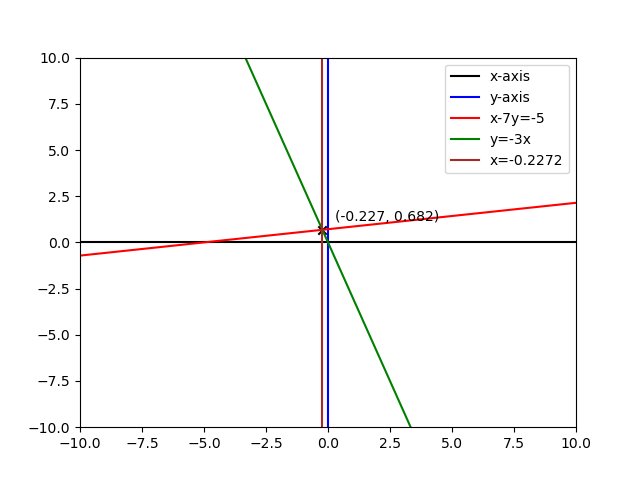
\includegraphics[width=\columnwidth]{./solutions/line_plane/47/Figure_1.png}
 \caption{graphical representation of systems of lines}
 \label{fig:linessolutions/line_plane/47/}
 \end{figure}
 Shown in Fig. \ref{fig:linessolutions/line_plane/47/} is the equation of the line parallel to the Y-axis drawn through the point of intersection of the lines.
